\section{Diagramas de conexiones}

A continuación, se describen los esquemas de conexión que definen la arquitectura experimental empleada en esta práctica. Estos diagramas proporcionan una representación detallada de la disposición física y eléctrica de los componentes, especificando las interconexiones entre los dispositivos de alimentación y los instrumentos de medición, lo cual resulta esencial para la correcta ejecución de los ensayos y la validez de los resultados obtenidos.

\subsection{Medición de resistencia}

 \begin{center}
        \begin{figure}[H]
        \centering  
        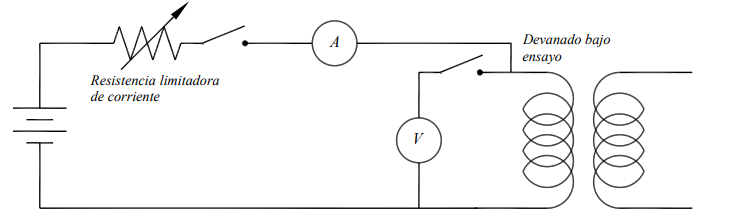
\includegraphics[scale=0.95]{imagenes/medicion de resistencia.png}
        \caption{Método del Voltímetro Amperímetro}
        \end{figure}
    \end{center} 

\subsection{Medición de relación de transformación}


 \begin{center}
        \begin{figure}[H]
        \centering  
        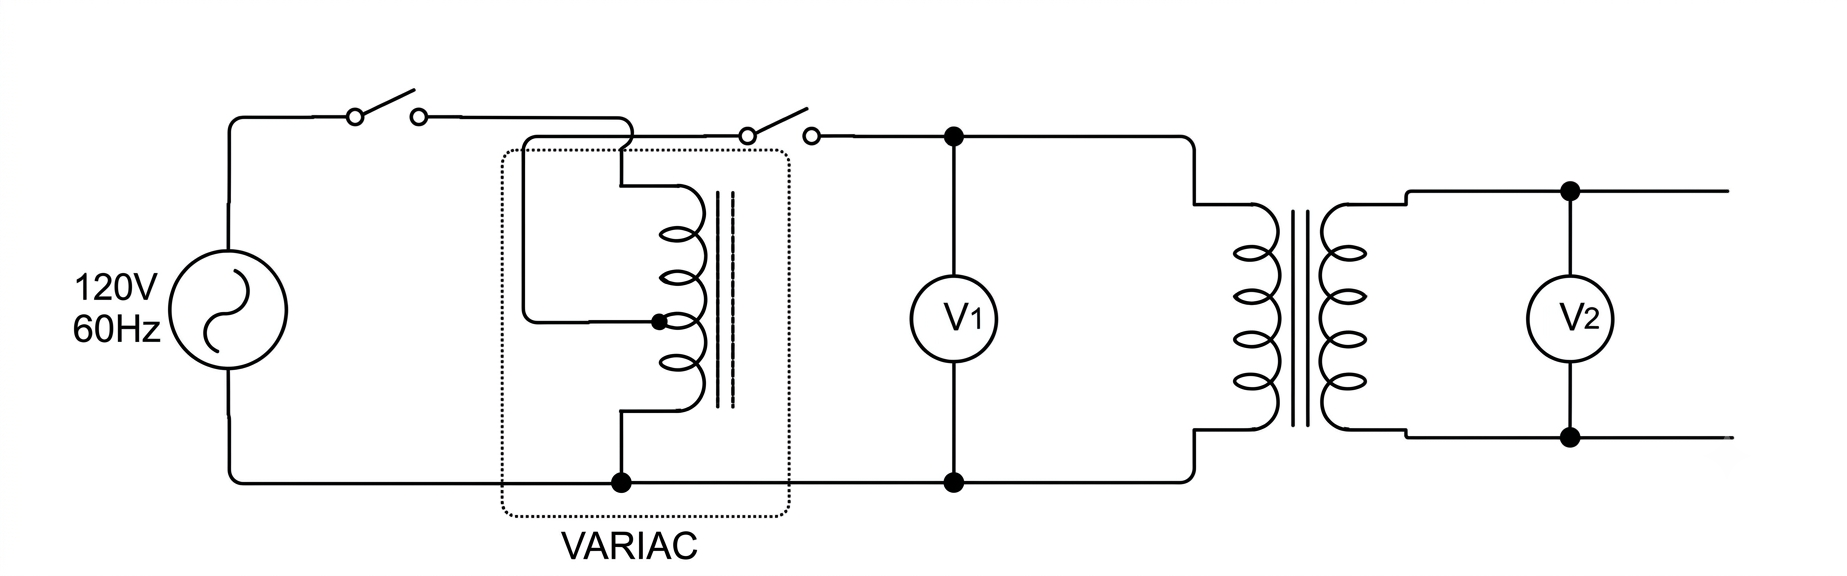
\includegraphics[scale=0.25]{imagenes/medicion de tranformador.png}
        \caption{Configuración experimental para la determinación de la relación de transformación.}
        \end{figure}
    \end{center} 
        
\subsection{Verificación de polaridad}

 \begin{center}
        \begin{figure}[H]
        \centering  
        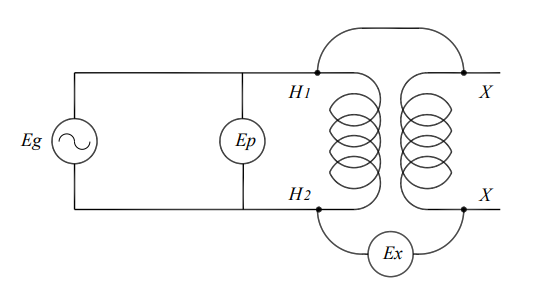
\includegraphics[scale=0.95]{imagenes/medicion de polaridad.png}
        \caption{Determinación de la polaridad de un transformador monofasico.}
        \end{figure}
    \end{center} 

\subsection{Ensayo de relación de las pérdidas debido a las cargas y tensiones de cortocircuito}



 \begin{center}
        \begin{figure}[H]
        \centering  
        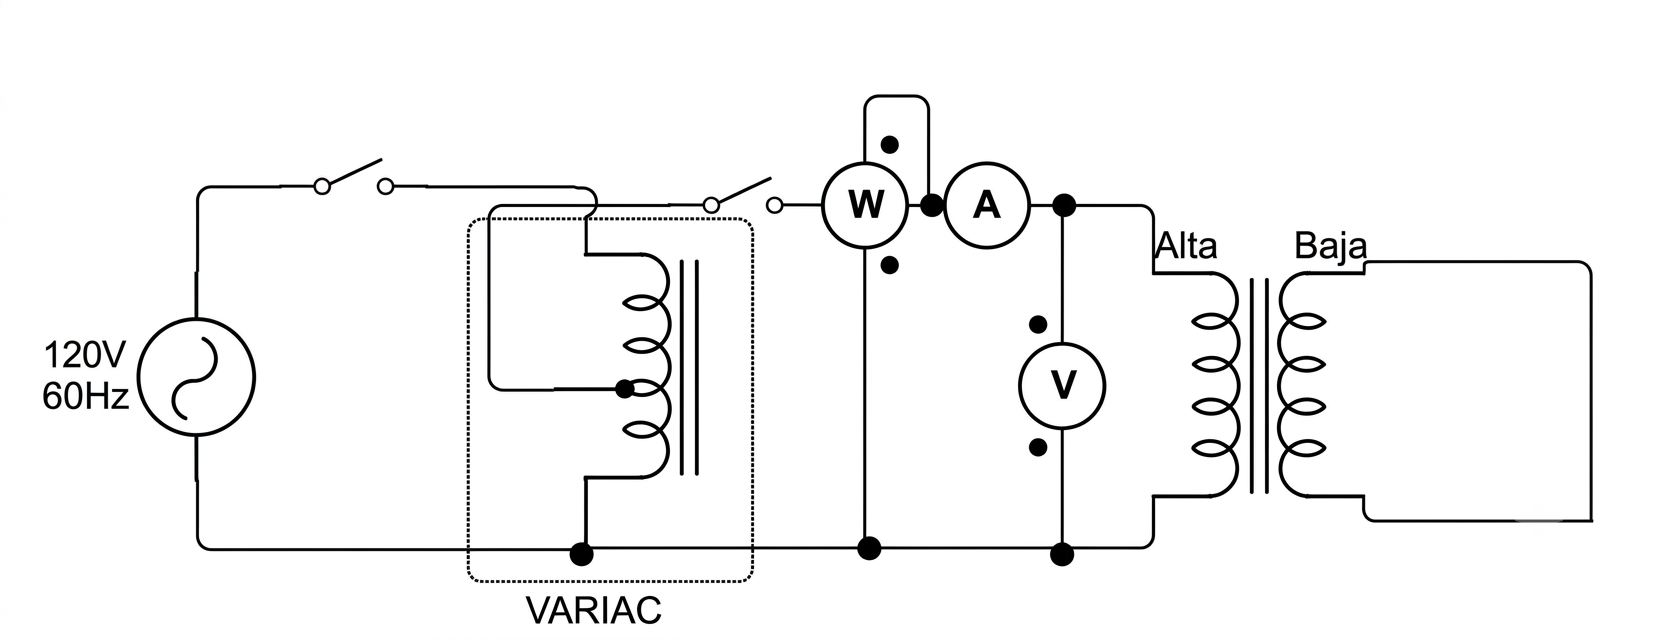
\includegraphics[scale=0.25]{imagenes/cortocircuito.png}
        \caption{ Esquema a utilizar en el ensayo de cortocircuito del transformador}
        \end{figure}
    \end{center} 

\subsection{Ensayo de la medición de las pérdidas y la corriente de vacío}


 \begin{center}
        \begin{figure}[H]
        \centering  
        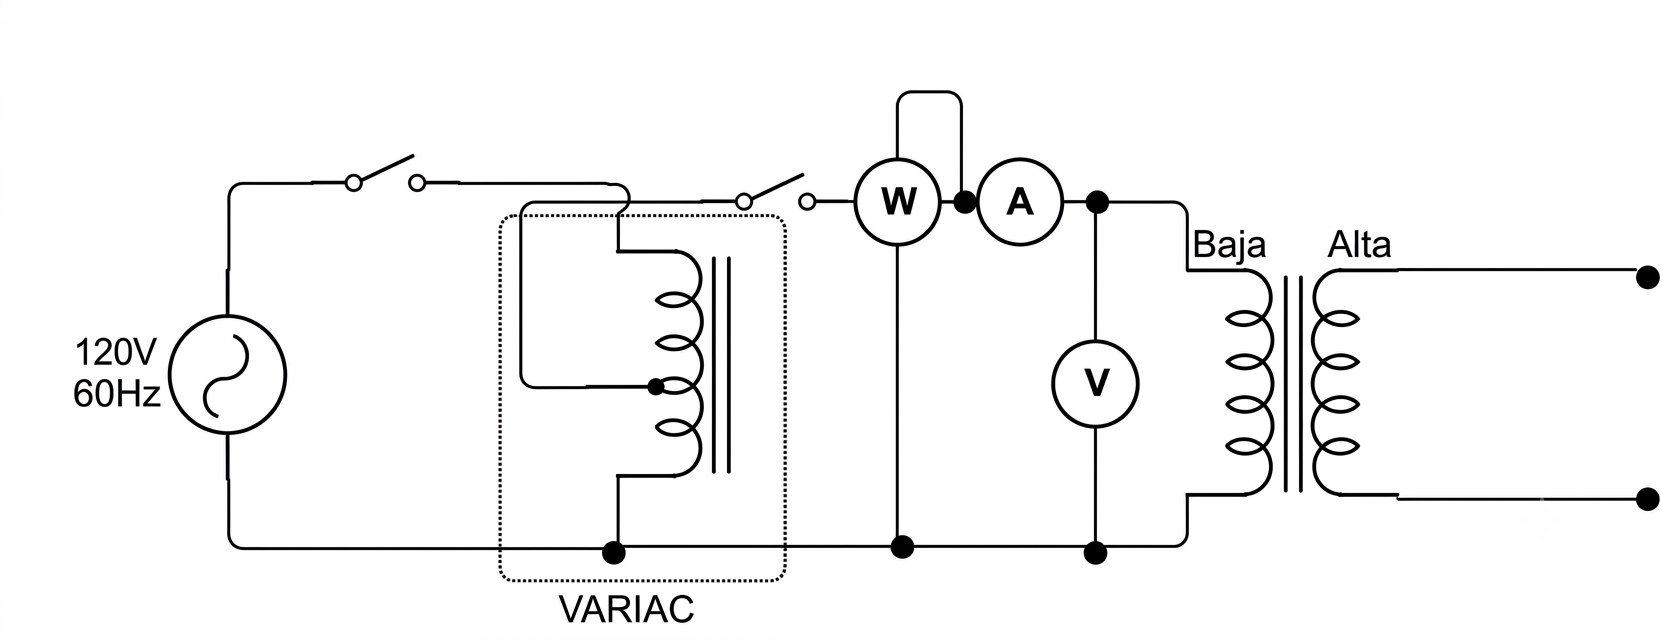
\includegraphics[scale=0.25]{imagenes/ciruito abierto.png}
        \caption{Esquema para la medicion de perdidas y determinación de la corriente de vacío.}
        \end{figure}
    \end{center}